% Kết quả thực nghiệm của phần B (chạy bằng src/train_models.py)
\subsubsection{Đánh giá đóng góp của từng nhóm đặc trưng (ablation)}\label{sec:ablation}

Để kiểm chứng các nhóm đặc trưng có thực sự hữu ích, phần B huấn luyện Random Forest (100 cây, siêu tham số tốt
nhất ở \cref{sec:rf}) và Ridge ($\alpha=1$) trên tập train với từng tổ hợp nhóm đặc trưng, rồi đo trên tập
validation ($h=24$).

\begin{table}[H]
\centering
\caption{Ablation nhóm đặc trưng -- sai số trên tập validation ($h=24$). In đậm: tốt nhất mỗi cột.}\label{tab:ablation}
\small
\setlength{\tabcolsep}{5pt}
\begin{tabular}{lrrrrr}
\toprule
& & \multicolumn{2}{c}{Random Forest} & \multicolumn{2}{c}{Ridge}\\
\cmidrule(lr){3-4}\cmidrule(lr){5-6}
Nhóm đặc trưng & Số ĐT & MAE (MW) & MAPE (\%) & MAE (MW) & MAPE (\%)\\
\midrule
Chỉ thời tiết & 11 & 3\,370 & 11.63 & 3\,507 & 12.12\\
Chỉ lag & 13 & 1\,825 & 6.36 & 2\,012 & 7.03\\
Chỉ lịch & 15 & 1\,798 & 6.06 & 2\,064 & 7.04\\
Lag + thời tiết & 24 & 1\,875 & 6.51 & 2\,024 & 7.04\\
Lịch + thời tiết & 26 & 1\,736 & 5.91 & 2\,074 & 7.07\\
Lịch + lag & 28 & 1\,545 & 5.29 & \textbf{1\,852} & \textbf{6.39}\\
\textbf{Tất cả (3 nhóm)} & 39 & \textbf{1\,536} & \textbf{5.28} & 1\,870 & 6.44\\
\bottomrule
\end{tabular}
\end{table}

\paragraph{Nhận xét.}
\begin{itemize}
  \item \textbf{Lịch và lag bổ trợ cho nhau}: mỗi nhóm riêng lẻ cho MAE khoảng 1\,800~MW, nhưng kết hợp thì
        giảm còn 1\,545~MW ($-14\%$). Lag cho biết \emph{mức} phụ tải gần đây; lịch cho biết \emph{hình dạng}
        trong ngày và ngày nghỉ --- điều mà lag 24 giờ không biết (ví dụ dự báo cho Thứ Hai bằng dữ liệu Chủ Nhật).
  \item \textbf{Thời tiết đứng riêng rất yếu} (MAPE 11.6\%) vì không biết giờ trong ngày, nhưng thêm vào
        lịch thì vẫn giảm MAE từ 1\,798 xuống 1\,736~MW với Random Forest. Khi đã có lag, phần lớn thông tin
        thời tiết đã ``nằm sẵn'' trong phụ tải hôm qua (nhiệt độ thay đổi chậm), nên đóng góp biên chỉ còn
        $\approx 9$~MW.
  \item \textbf{Với Ridge, thêm thời tiết làm tệ đi nhẹ} (1\,852 $\to$ 1\,870~MW): quan hệ nhiệt độ--phụ tải
        phụ thuộc giờ trong ngày (\cref{fig:eda}, ô 2) mà mô hình tuyến tính cộng tính không biểu diễn được,
        nên các biến thời tiết chủ yếu thêm nhiễu. Đây là một lý do mô hình cây vượt trội ở \cref{sec:compare-c}.
\end{itemize}
Bộ đặc trưng đầy đủ 39 biến được giữ làm mặc định vì tốt nhất với mô hình phi tuyến (cũng là họ mô hình
boosting của phần D), còn Ridge tự co các hệ số thừa nhờ điều chuẩn.

\subsubsection{Độ quan trọng của đặc trưng}\label{sec:importance}

\Cref{fig:perm-imp} cho thấy \emph{permutation importance} của Random Forest: mức tăng MAE trên tập validation
khi xáo trộn ngẫu nhiên một cột (5 lần lặp). Khác với độ quan trọng theo độ giảm impurity --- vốn thiên vị các
biến liên tục/nhiều giá trị~\cite{strobl2007bias} --- permutation importance đo trực tiếp đóng góp vào sai số
trên dữ liệu chưa thấy.

\begin{figure}[H]
\centering
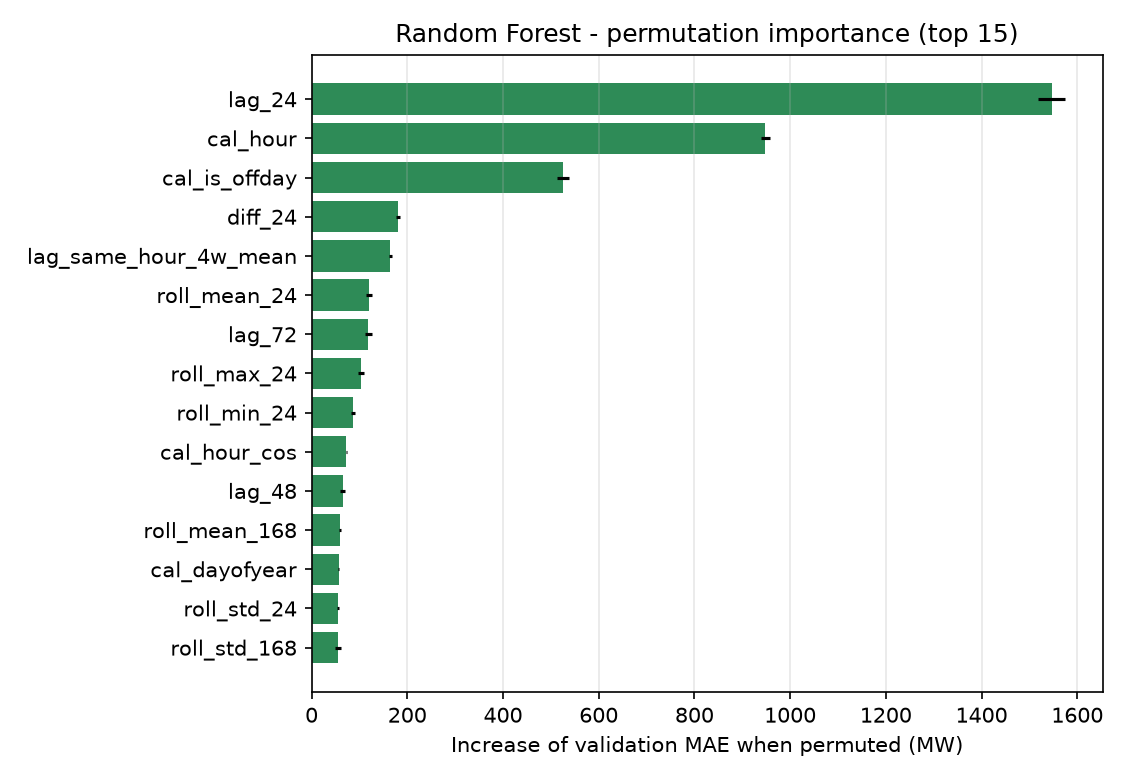
\includegraphics[width=0.8\linewidth]{b_feature_importance_rf.png}
\caption{Permutation importance (top 15) của Random Forest trên tập validation.}
\label{fig:perm-imp}
\end{figure}

Ba đặc trưng quan trọng nhất đến từ cả ba ý tưởng chính của phần B:
\code{lag_24} (+1\,546~MW khi bị xáo trộn), \code{cal_hour} (+948~MW) và \code{cal_is_offday} (+525~MW) ---
chính là biến ngày nghỉ tự xây dựng (cuối tuần \emph{hoặc} lễ). Tiếp theo là các đặc trưng lag phái sinh
(\code{diff_24}, \code{lag_same_hour_4w_mean}, \code{roll_mean_24}). Chỉ số impurity lại xếp \code{cal_hour}
cao nhất (0.45 so với 0.14 của \code{lag_24}), minh họa sự thiên vị nói trên.

\subsubsection{Ảnh hưởng của chân trời dự báo}\label{sec:horizon}

\begin{table}[H]
\centering
\caption{So sánh dự báo trước 1 giờ và trước 24 giờ (tập validation, cùng bộ đặc trưng và siêu tham số).}\label{tab:horizon}
\begin{tabular}{llrrr}
\toprule
Chân trời & Mô hình & MAE (MW) & RMSE (MW) & MAPE (\%)\\
\midrule
\multirow{3}{*}{$h=1$} & Ngây thơ $y_{t-1}$ & 1\,115 & 1\,507 & 3.91\\
 & Ridge & 405 & 677 & 1.42\\
 & Random Forest & \textbf{310} & \textbf{531} & \textbf{1.07}\\
\midrule
\multirow{3}{*}{$h=24$} & Ngây thơ $y_{t-24}$ & 2\,429 & 3\,507 & 8.43\\
 & Ridge & 1\,856 & 2\,513 & 6.39\\
 & Random Forest & \textbf{1\,536} & \textbf{2\,282} & \textbf{5.28}\\
\bottomrule
\end{tabular}
\end{table}

Khi được dùng $y_{t-1}$, mọi mô hình tốt hơn khoảng 5 lần. Điều này cho thấy hai điều: (i) chọn chân trời
là quyết định thiết kế quan trọng nhất và \textbf{phải được nêu rõ} khi so sánh với các kết quả khác --- nhiều
notebook công khai trên bộ dữ liệu này dùng lag 1 giờ nên có sai số thấp hơn nhiều; (ii) với $h=1$, Random
Forest đạt MAPE 1.07\%, xấp xỉ dự báo của TSO (1.05\%), gợi ý rằng dự báo TSO trong dữ liệu được cập nhật gần
thời gian thực chứ không phải dự báo ngày tới thuần túy (\cref{sec:baselines}).

\subsubsection{Một quan sát về chất lượng dữ liệu}\label{sec:data-quirk}

Khi phân tích sai số lớn nhất (\cref{sec:error-analysis}), phần B phát hiện chuỗi phụ tải có \textbf{tính mùa vụ
theo tuần yếu bất thường}: tự tương quan của phụ tải trung bình ngày ở độ trễ 7 ngày chỉ là 0.27 (nhỏ hơn
cả độ trễ 1 ngày, 0.37), và phụ tải trung bình Chủ Nhật chỉ thấp hơn Thứ Tư khoảng 12\%. Có những ngày cuối tuần
mang mức phụ tải của ngày làm việc (ví dụ Thứ Bảy 02/06/2018 trung bình 34\,328~MW, cao hơn mọi ngày trong
tuần trước đó) và ngược lại (Thứ Ba 05/06/2018 chỉ 23\,287~MW). Cột \code{total load forecast} của TSO cũng
bám đúng các bất thường này. Đây là đặc tính của dữ liệu nguồn chứ không phải lỗi của pipeline (các mốc thời
gian và tính liên tục theo giờ đã được kiểm tra), nhưng nó giới hạn độ chính xác mà các đặc trưng lịch có thể
mang lại. Nhóm đề xuất phần A kiểm tra thêm với dữ liệu gốc từ ENTSO-E/REE.
